\documentclass{beamer}
\usepackage{CJK}
\usepackage{picinpar,graphicx}
\usefonttheme[onlymath]{serif}
\usepackage[greek,english]{babel}
\usepackage{bm}

\begin{document}
\begin{CJK}{UTF8}{song}

\begin{frame}[allowframebreaks]
\frametitle{整数规划}

在很多应用领域中,最优化问题需要额外要求全部或部分自变量取整数,这类问题又称为整数规划.
\begin{figure}
\centering
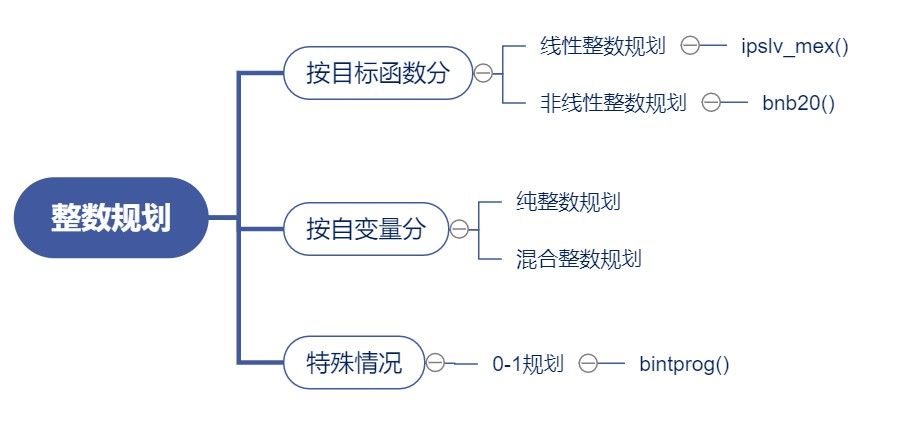
\includegraphics[width=0.88\textwidth]{zsgh.jpg}
\caption{整数规划的划分}
\end{figure}
\end{frame}

\begin{frame}[allowframebreaks]
\frametitle{整数线性规划问题的求解}

\begin{equation}
\begin{array}{c}
\min f^{T} x \\
x \in Z \text { s.t.}\left\{\begin{array}{c}
A x \leq B \\
A_{e q} x=B_{e q} \\
x_{m} \leq x \leq x_{M}
\end{array}\right.
\end{array}
\end{equation}

之前MATLAB没有提供整数线性规划的函数,常用有代表性的Michel Berkelaar等人开发的lpslv包.
\begin{equation}
[x, h o w]=i p s l v_{-} \operatorname{mex}\left(A, B, f, \text {intlist}, x_{m}, x_{M}, \text {ctype}\right)
\end{equation}
\end{frame}

\begin{frame}[allowframebreaks]
\frametitle{一般非线性整数规划问题与求解}

实际应用中经常需要求解非线性整数规划或混合规划问题,常用求解函数是基于分枝定界算法编写的bnb20函数.
\begin{equation}
[e r r, f, x]=b n b 20\left(f u n, x_{0}, \text { intlist }, x_{m}, x_{M}, A, B, A_{e q}, B_{e q}\right)
\end{equation}
该函数主要调用的是最优化工具箱函数.
\end{frame}

\begin{frame}[allowframebreaks]
\frametitle{0-1规划问题求解}

MATLAB提供了用来求解0-1线性规划问题的函数bintprog,但不能直接求解非线性0-1规划问题.
\begin{equation}
x=\operatorname{bintprog}\left(f, A, B, A_{e q}, B_{e q}\right)
\end{equation}
免费的MAILAB函数求解非线性混合整数规划的功能不是很强大,基于MATLAB的商业软件TOMLAB更复杂,但功能也更加全面且出色.
\end{frame}

\begin{frame}[allowframebreaks]
\frametitle{应用举例}

MATLAB后续版本中更新了MILP函数,可以求解混合线性整数规划问题.
\begin{equation}
x=\operatorname{intlinprog}\left(f, \text {intcon,} A, B, A_{e q}, B_{e q}, x_{m}, x_{M}\right)
\end{equation}
以解下面的优化问题为例
\begin{equation}
\begin{array}{c}
\min \left(-2 x_{1}-x_{2}-4 x_{3}-3 x_{4}-x_{5}\right) \\
2 x_{2}+x_{3}+4 x_{4}+2 x_{5} \leq 54 \\
3 x_{1}+4 x_{2}+5 x_{3}-x_{4}-x_{5} \leq 62 \\
x_{1} \geq 0, x_{2} \geq 0, x_{3} \geq 3.32, x_{4} \geq 0.678, x_{5} \geq 2.57
\end{array}
\end{equation}
\end{frame}

\begin{frame}[allowframebreaks]
\frametitle{结果}

\begin{equation}
\begin{array}{c}
\min \left(-2 x_{1}-x_{2}-4 x_{3}-3 x_{4}-x_{5}\right) \\
2 x_{2}+x_{3}+4 x_{4}+2 x_{5} \leq 54 \\
3 x_{1}+4 x_{2}+5 x_{3}-x_{4}-x_{5} \leq 62 \\
x_{1} \geq 0, x_{2} \geq 0, x_{3} \geq 3.32, x_{4} \geq 0.678, x_{5} \geq 2.57
\end{array}
\end{equation}
\begin{figure}
\centering
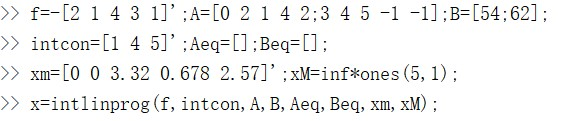
\includegraphics[width=0.88\textwidth]{test1.jpg}
\caption{参数输入}
\end{figure}

\begin{figure}
\centering
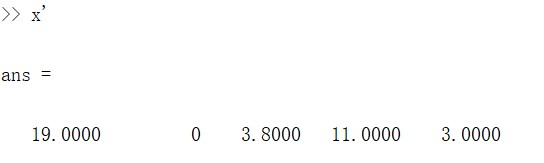
\includegraphics[width=0.72\textwidth]{ans1.jpg}
\caption{算例结果}
\end{figure}
时间客观上是连续的,但社会时间是离散的,整数规划相较于连续优化问题,看似是简化了条件,实际的解决难度却并没有降低,并且其在交通、能源等诸多实际领域中具有更高的应用价值。但是也不能否定了连续优化的作用,科学的本质便是从简到难,先把简单问题研究透彻,再把复杂问题简化为求解一个个简单的问题.
\end{frame}

\end{CJK}
\end{document}